\documentclass[12pt,a4paper]{amsart}
\usepackage[a4paper,margin=1in]{geometry}
\usepackage[euler-digits]{eulervm}
\usepackage{tikz}
\usetikzlibrary{calc}

\begin{document}
\section*{$C_3$.}
\begin{center}
  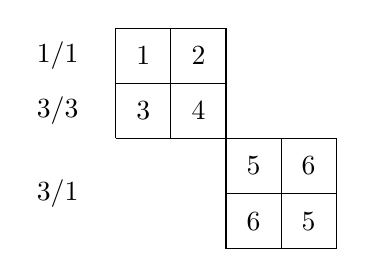
\begin{tikzpicture}[xscale=0.7,yscale=-0.7]
    \draw[shift={(0.5,0.5)}](0,0) grid (2,2);
    \draw[shift={(0.5,0.5)}](2,2) grid (4,4);
    \node[anchor=east] at (0,1) {$1/1$};
    \node[anchor=east] at (0,2) {$3/3$};
    \node[anchor=east] at (0,3.5) {$3/1$};
    \foreach \i in {1,...,4}
      \node[anchor=center] at ({mod(\i-1,2)+1}, {int((\i+1)/2)}) {$\i$};
    \node[anchor=center] at (3, 3) {$5$};
    \node[anchor=center] at (4, 4) {$5$};
    \node[anchor=center] at (3, 4) {$6$};
    \node[anchor=center] at (4, 3) {$6$};
      \end{tikzpicture}
%\end{center}
\quad
%\begin{center}
  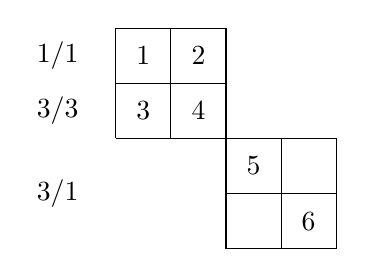
\begin{tikzpicture}[xscale=0.7,yscale=-0.7]
    \draw[shift={(0.5,0.5)}](0,0) grid (2,2);
    \draw[shift={(0.5,0.5)}](2,2) grid (4,4);
    \node[anchor=east] at (0,1) {$1/1$};
    \node[anchor=east] at (0,2) {$3/3$};
    \node[anchor=east] at (0,3.5) {$3/1$};
    \foreach \i in {1,...,4}
      \node[anchor=center] at ({mod(\i-1,2)+1}, {int((\i+1)/2)}) {$\i$};
    \node[anchor=center] at (3, 3) {$5$};
    \node[anchor=center] at (4, 4) {$6$};
      \end{tikzpicture}
\end{center}

\scriptsize
\begin{align*}
M &=  
\left(\begin{array}{rrrrrr}%
3&.&.&.&.&.\\%
1&1&.&.&.&.\\%
1&.&1&.&.&.\\%
\!\!\!^1\!/\!_3&\!\!\!^1\!/\!_3&\!\!\!^1\!/\!_3&\!\!\!^1\!/\!_3&.&.\\%
1&.&.&.&1&.\\%
1&.&.&.&.&1\\%
\end{array}\right)%
\cdot 
\left(\begin{array}{rrrrrr}%
1&.&.&.&.&.\\%
.&1&.&.&.&.\\%
.&.&2&.&.&.\\%
.&.&.&2&.&.\\%
.&.&.&.&1&.\\%
.&.&.&.&.&1\\%
\end{array}\right)%
\cdot
\left(\begin{array}{rrrrrr}%
1&.&.&.&.&.\\%
.&1&.&.&.&.\\%
.&.&1&.&.&.\\%
.&.&.&1&.&.\\%
.&.&.&1&1&.\\%
.&.&.&1&.&1\\%
\end{array}\right) \\
M &= 
\left(\begin{array}{rrrrrr}%
3&.&.&.&.&.\\%
1&1&.&.&.&.\\%
1&.&2&.&.&.\\%
\!\!\!^1\!/\!_3&\!\!\!^1\!/\!_3&\!\!\!^2\!/\!_3&\!\!\!^2\!/\!_3&.&.\\%
1&.&.&1&1&.\\%
1&.&.&1&.&1\\%
\end{array}\right)%\\
\quad
  M^{-1} =
\left(\begin{array}{rrrrrr}%
\frac13&.&.&.&.&.\\%
-\frac13&1&.&.&.&.\\%
-\frac{1}{6}&.&\frac12&.&.&.\\%
\frac{1}{6}&-\frac12&-\frac12&3/2&.&.\\%
-\frac12&\frac12&\frac12&-3/2&1&.\\%
-\frac12&\frac12&\frac12&-3/2&.&1\\%
\end{array}\right)%
\end{align*}


\begin{align*}
\left(\begin{array}{rrrr}
3&.&.&.\\
.&.&.&.\\
.&.&.&.\\
.&.&.&.\\
\end{array}\right)
\quad
\left(\begin{array}{rrrr}
1&1&.&.\\
.&.&.&.\\
.&.&.&.\\
.&.&.&.\\
\end{array}\right)
\quad
\frac13\left(\begin{array}{rrrr}
3&.&.&.\\
2\cdot3&.&.&.\\
.&.&.&.\\
.&.&.&.\\
\end{array}\right)
\quad
\frac13\left(\begin{array}{rrrr}
1&1&.&.\\
2\cdot1&2\cdot1&.&.\\
.&.&.&.\\
.&.&.&.\\
\end{array}\right)
\end{align*}

\begin{align*}
\left(\begin{array}{rrrr}
1&.&.&.\\
.&1&.&.\\
.&.&1&.\\
.&.&.&1\\
\end{array}\right)
\quad
\left(\begin{array}{rrrr}
1&.&.&.\\
.&1&.&.\\
.&.&.&1\\
.&.&1&.\\
\end{array}\right)
\end{align*}

\end{document}
